% Useful packages
\documentclass[12pt]{article}
\usepackage[a4paper, left=0.75in, right=0.75in, top=0.75in, bottom=0.75in]{geometry}
\usepackage{amsmath}
\usepackage{amssymb}
\usepackage{float}
\usepackage{tabularx}
\usepackage{array}
\usepackage{multirow}
\usepackage{booktabs}
\usepackage{minted}
\usepackage{xcolor}
\usepackage{enumitem}
\usepackage{hyperref}
\usepackage{graphicx}
\usepackage{longtable}
\usepackage{adjustbox}
\usepackage{textcomp}
\usepackage{subcaption}
\usepackage{mathtools}


% chktex-file 13
% chktex-file 24
% chktex-file 36
% chktex-file 44


% Customizations
\definecolor{inputGray}{HTML}{f8f8f8}
\definecolor{outGray}{HTML}{dfdfdf}


\title{%
    Machine Learning in Computational Biology \\
    \Large Assignment 1 
    }
\author{%
    Konstantinos Konstantinidis \\
    Student number: 7115152400017
    }

\begin{document}

\maketitle

\vspace{0.5in}

\textbf{\underline{Repo:}} The repository for this assignment can be found here: \\
\url{https://github.com/KonsKons26/Assignment-1}

\vspace{0.5in}

% Table of contents
\tableofcontents
\clearpage

% \clearpage
%%%%%%%%%%%%%%%%%%%%%%%%%%%%%%%%%%%%%%%%%%%%%%%%%%%%%%%%%%%%%%%%%%%%%%%%%%%%%%%%%%%%
\section{Data Exploration}

\subsection{Preprocessing}
Befor beginning with any machine learning task, we need to inspect the data and
perform some rudimentary preprocessing steps. The dataset is provided in two
\texttt{.csv} files, one for developing and one for validating the models. Both
datasets contained no missing values, but they contained some columns with
metadata, namely \texttt{Project ID}, \texttt{Experiment Type}, and \texttt{%
Disease MESH ID}. These columns were removed from both datasets. Finally, the
values in the \texttt{Sex} column were converted to binary values, where \texttt{%
male} was set to $0$ and \texttt{female} to $1$.


\subsection{Data Exploration}
All analyses were performed on the \textbf{development} dataset.

First, I decided to plot the distribution of the BMI values. The distribution is
shown in Figure~\ref{fig:bmi_hist_by_sex}. The histogram contains the BMI values,
while the \texttt{kde} lines show their distribution. The distribution does not seem
to be normal, as it is skewed to the right and when the values for both sexes are
combined, the distribution seems bimodal.

\begin{figure}[H]
    \centering
    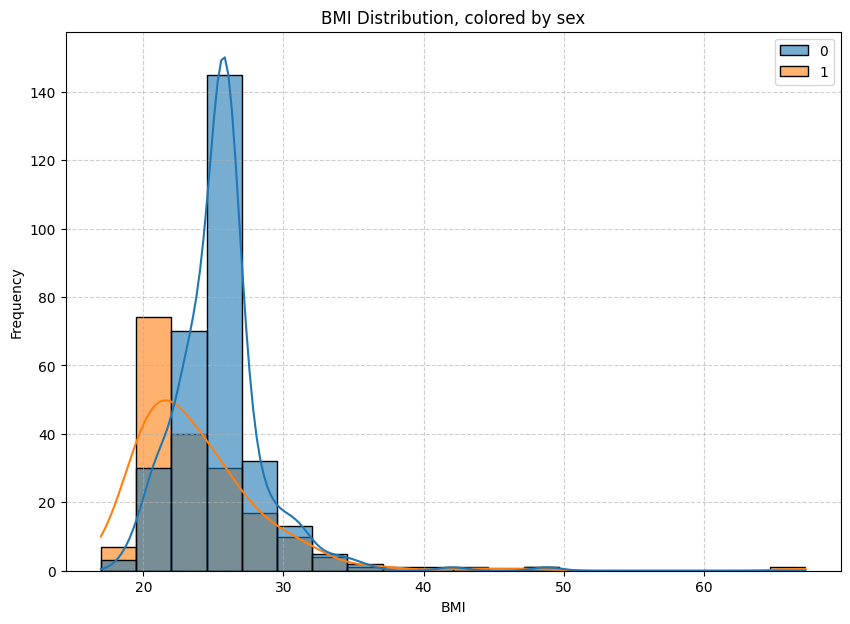
\includegraphics[width=0.75\textwidth]{ims/bmi_hist_by_sex.png}
    \caption{Histogram with a \texttt{kde} lines, colored by sex.}
    \label{fig:bmi_hist_by_sex}
\end{figure}

Another really interesting plot is the one showing the number of zeros in each
feature and the mean \texttt{BMI} when the bacterial concentrations are non-zero.
The plot is shown in Figure~\ref{fig:zeros}. The plot shows that a great number of
bacteria have a lot of zero values. Also, the mean BMI (when ignoring the zeros)
diverges a lot from the mean value of the whole dataset for the bacteria that have a
lot of zeros. This might indicate that these bacteria are highly correlated with the
\texttt{BMI} values.

\begin{figure}[H]
    \centering
    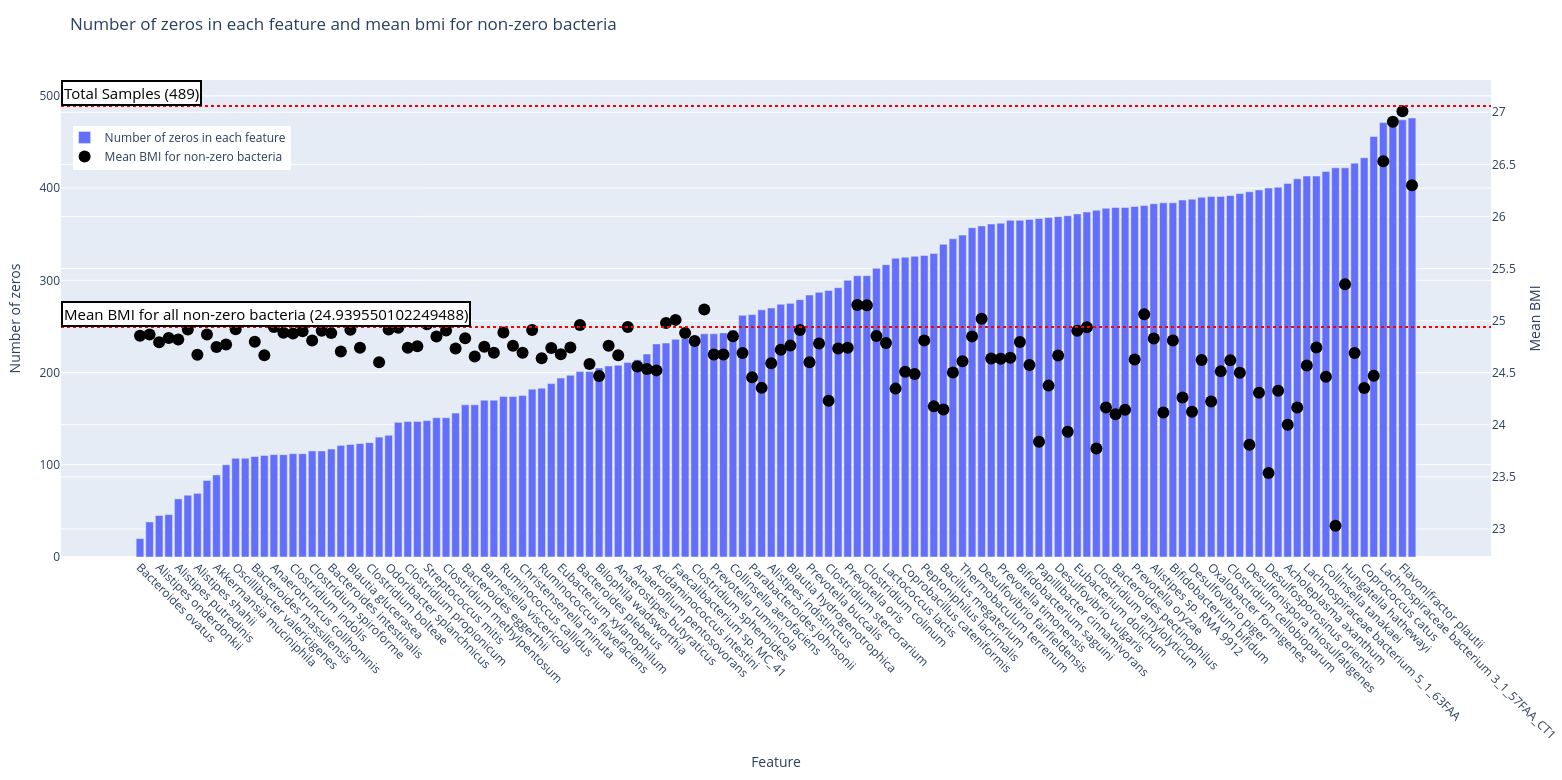
\includegraphics[width=0.95\textwidth]{ims/zeros_and_mean_for_non_zeros.png}
    \caption{Barplot (sorted) showing the number of zeros in each bacterium and the
    mean \texttt{BMI} when the bacteria are not zero.}
    \label{fig:zeros}
\end{figure}

A good way to grasp the feature space is to plot the mean, min, and max BMI
for each feature, as show in Figure~\ref{fig:feature_spans}. We can see that the
mean values of almost all bacteria lie around $0$, they have very small IQR's and
very few outliers. A MinMax normalization would make the feature space very sparsely
populated, so it seems like a bad choice. On the other hand, a standardization
seems more optimal; even if it might lead to negative values which make no sense
when talking about bacterial concentrations, our models will not mind. A plot
in similar spirit is shown below (Figure~\ref{fig:feature_standardized}).

\begin{figure}[H]
    \centering
    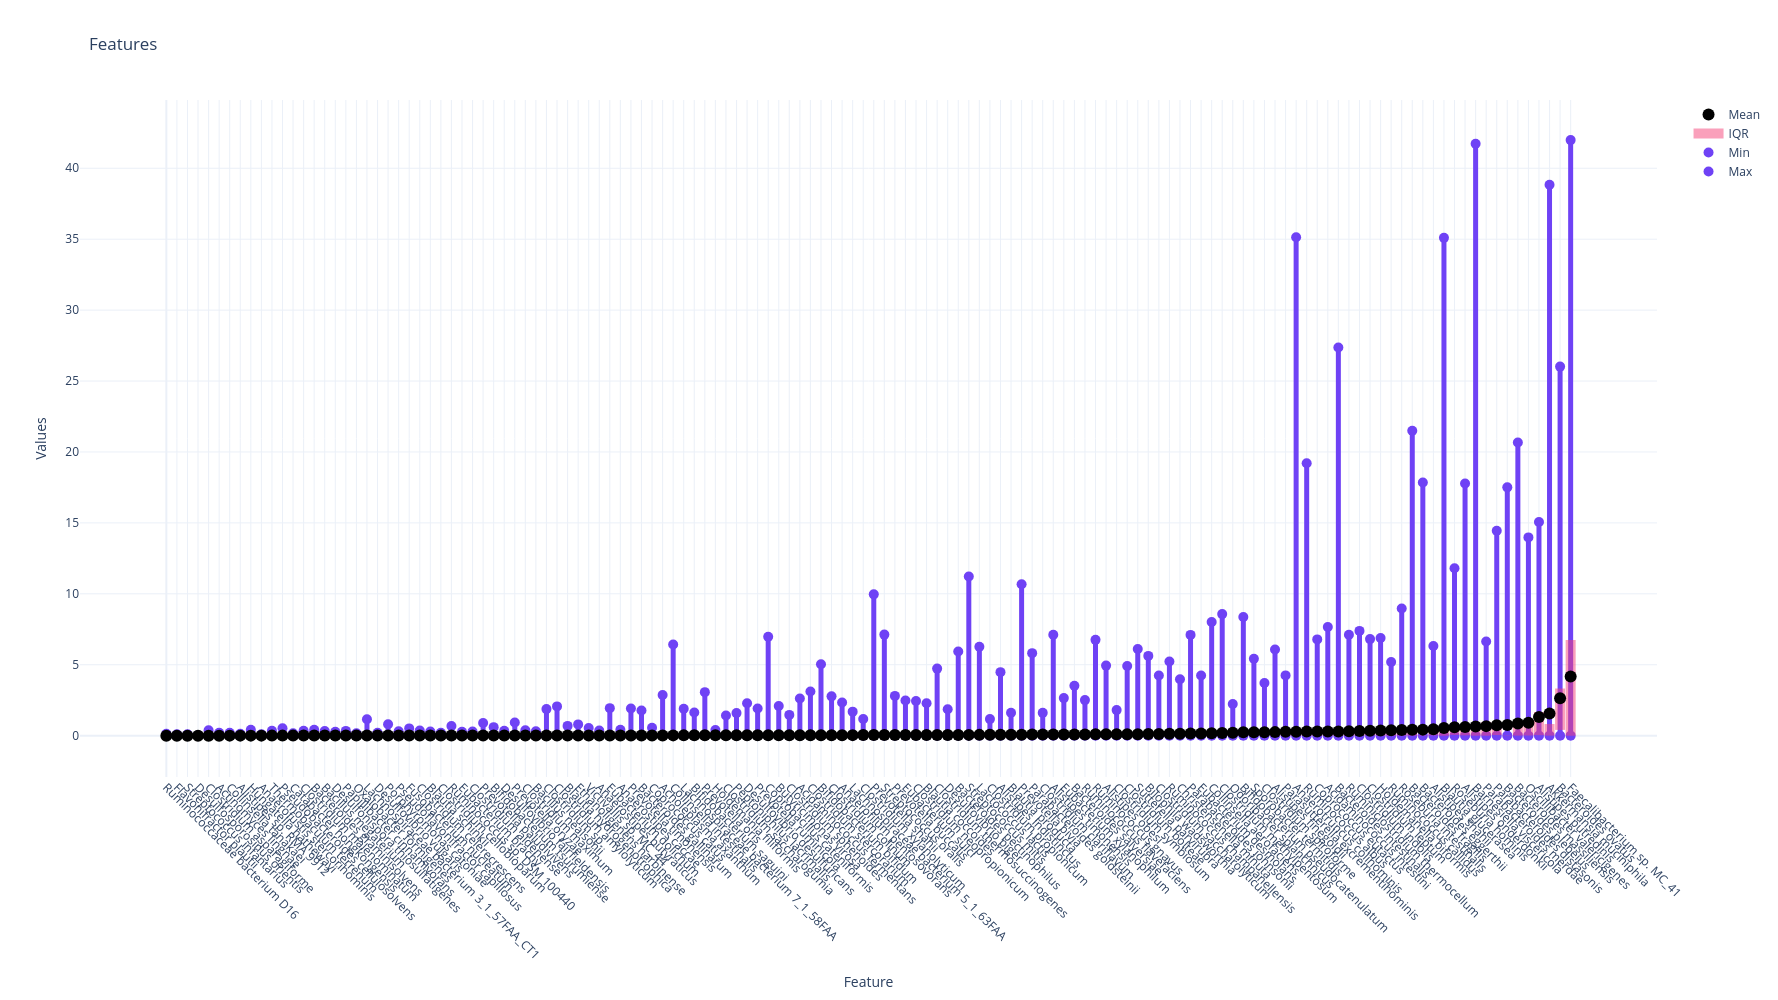
\includegraphics[width=\textwidth]{ims/features_spans.png}
    \caption{Feature spans: Mean, minimum and maximum, and Inter-Quantile Range IQR
    of each feature, (black circles, purple sticks, transparent pink bars
    respectively). Features sorted by ascending mean values.}
    \label{fig:feature_spans}
\end{figure}

\begin{figure}[H]
    \centering
    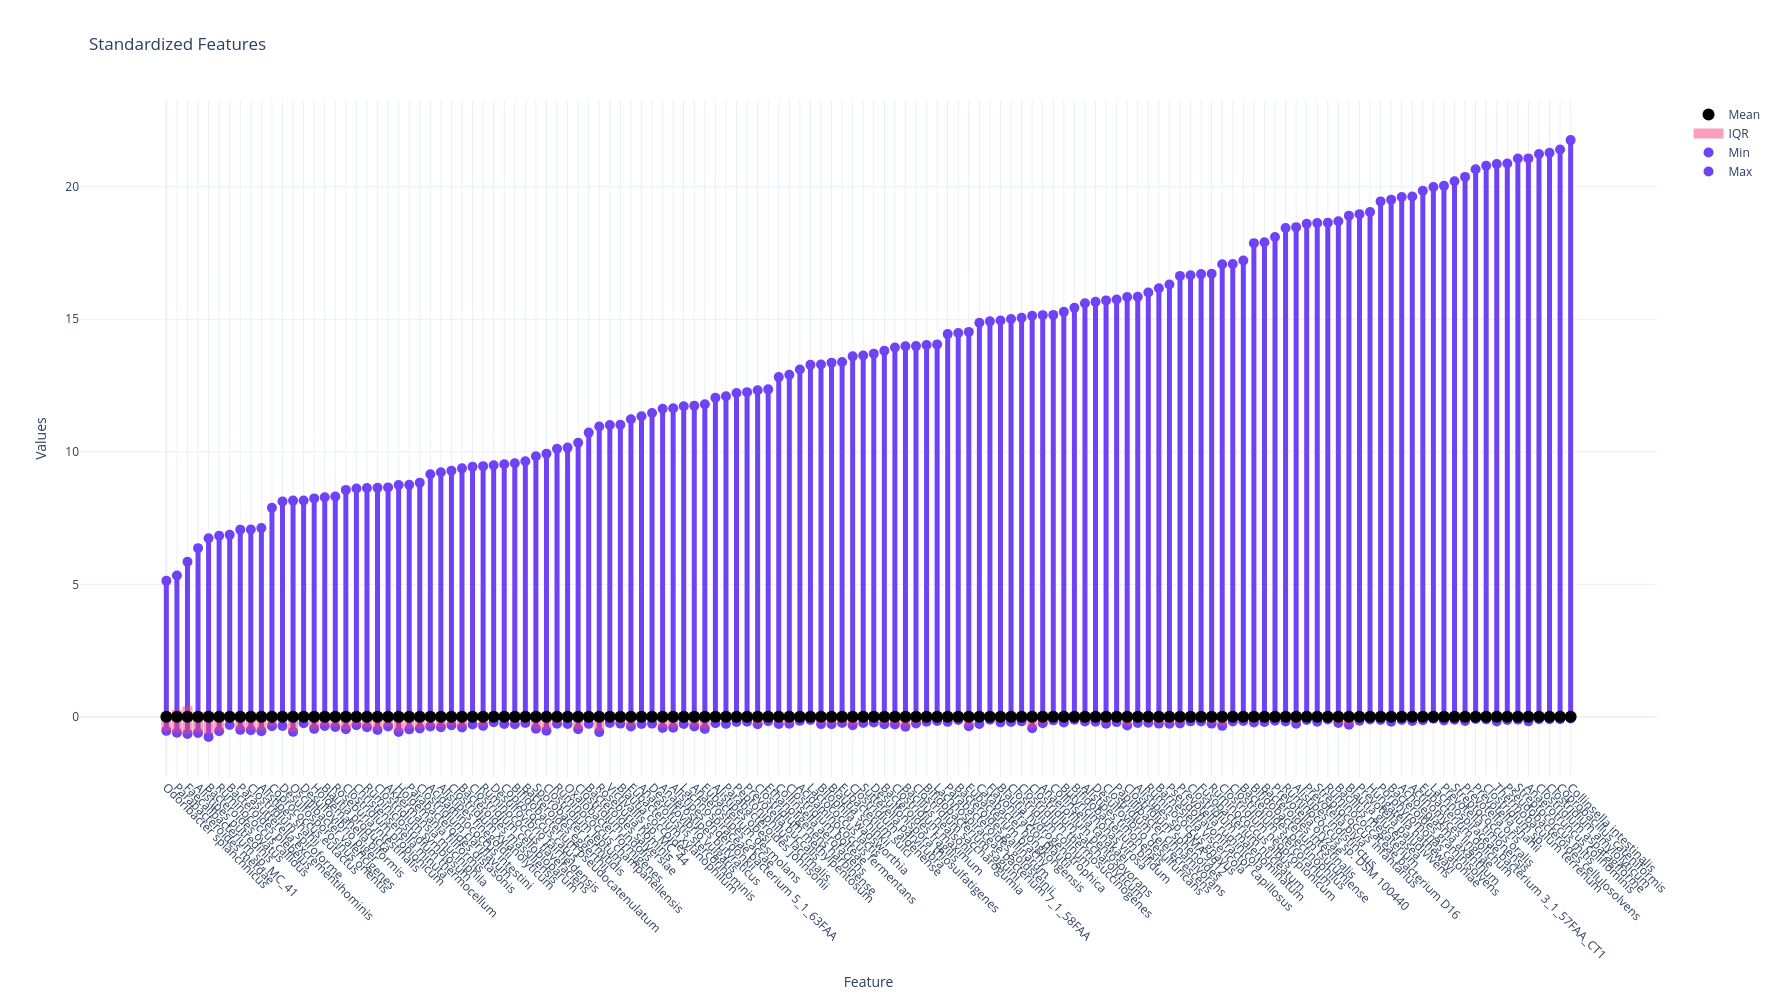
\includegraphics[width=\textwidth]{ims/features_standardized.png}
    \caption{Features --- Standardized: Mean, minimum and maximum, and Inter-Quantile
    Range IQR of each feature, (black circles, purple sticks, transparent pink bars
    respectively). Features sorted by ascending max values.}
    \label{fig:feature_standardized}
\end{figure}

Another importand metric when aiming for a regression model is to check the
correlation of the features with the target values. Pearson's correlation
coefficient measure linear relationship between the two variables, while
Spearman's and Kendall's can capture non-linear relationships, as long as they
are monotonic. In either case though, our dataset does not show any type of
correlation (Figure~\ref{fig:corrs}).

\begin{figure}[H]
    \centering
    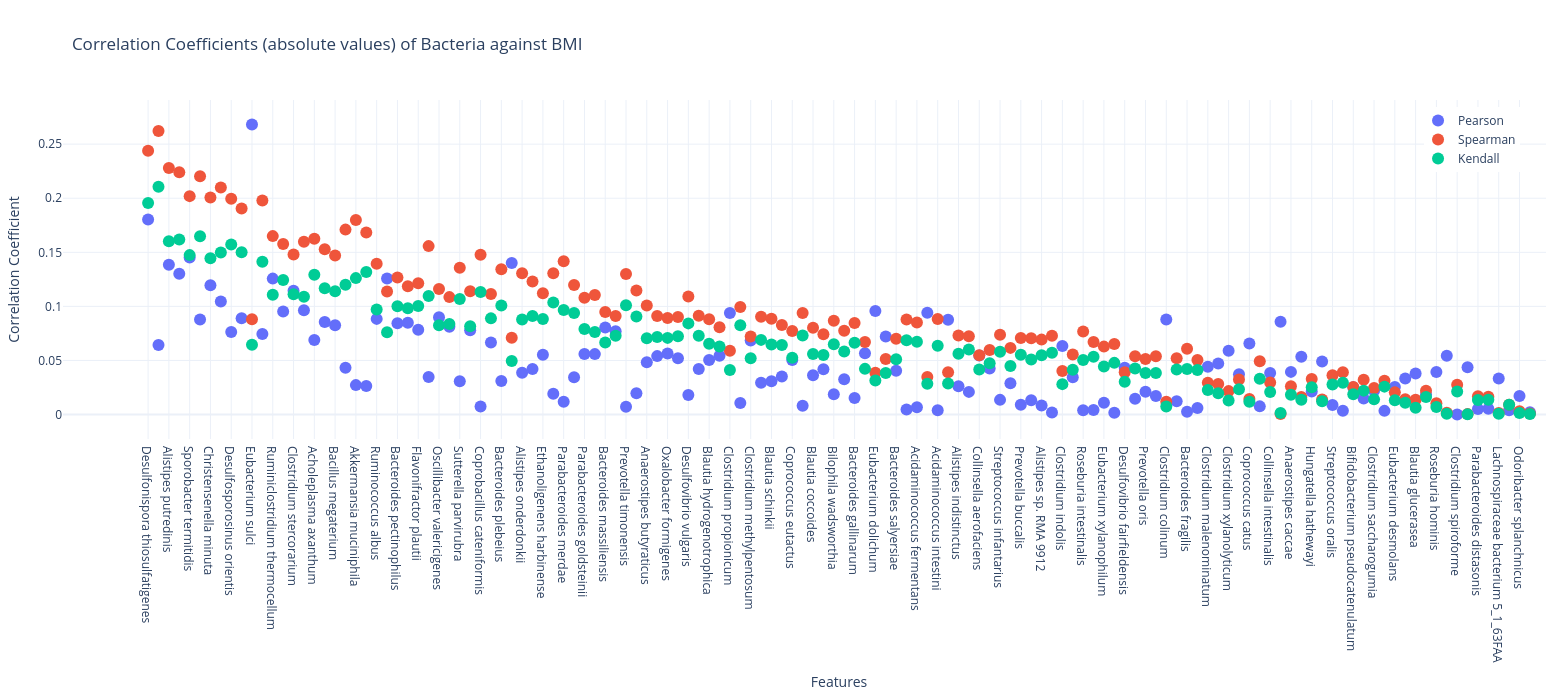
\includegraphics[width=\textwidth]{ims/corr_coeffs.png}
    \caption{Pearson's r, Spearman's $\rho$, and Kendall's $\tau$ absolute
    correlations of the bacteria with BMI (blue, red, and green respectively),
    sorted by descending order.}
    \label{fig:corrs}
\end{figure}

Taking the $5$ most correlated bacteria with BMI, and plotting them against each
other in a pairplot (Figure~\ref{fig:corrs_top_5}), we can see that they are
highly uncorrelated, indicating that they at least will carry different information
to the regression problem.

\begin{figure}[H]
    \centering
    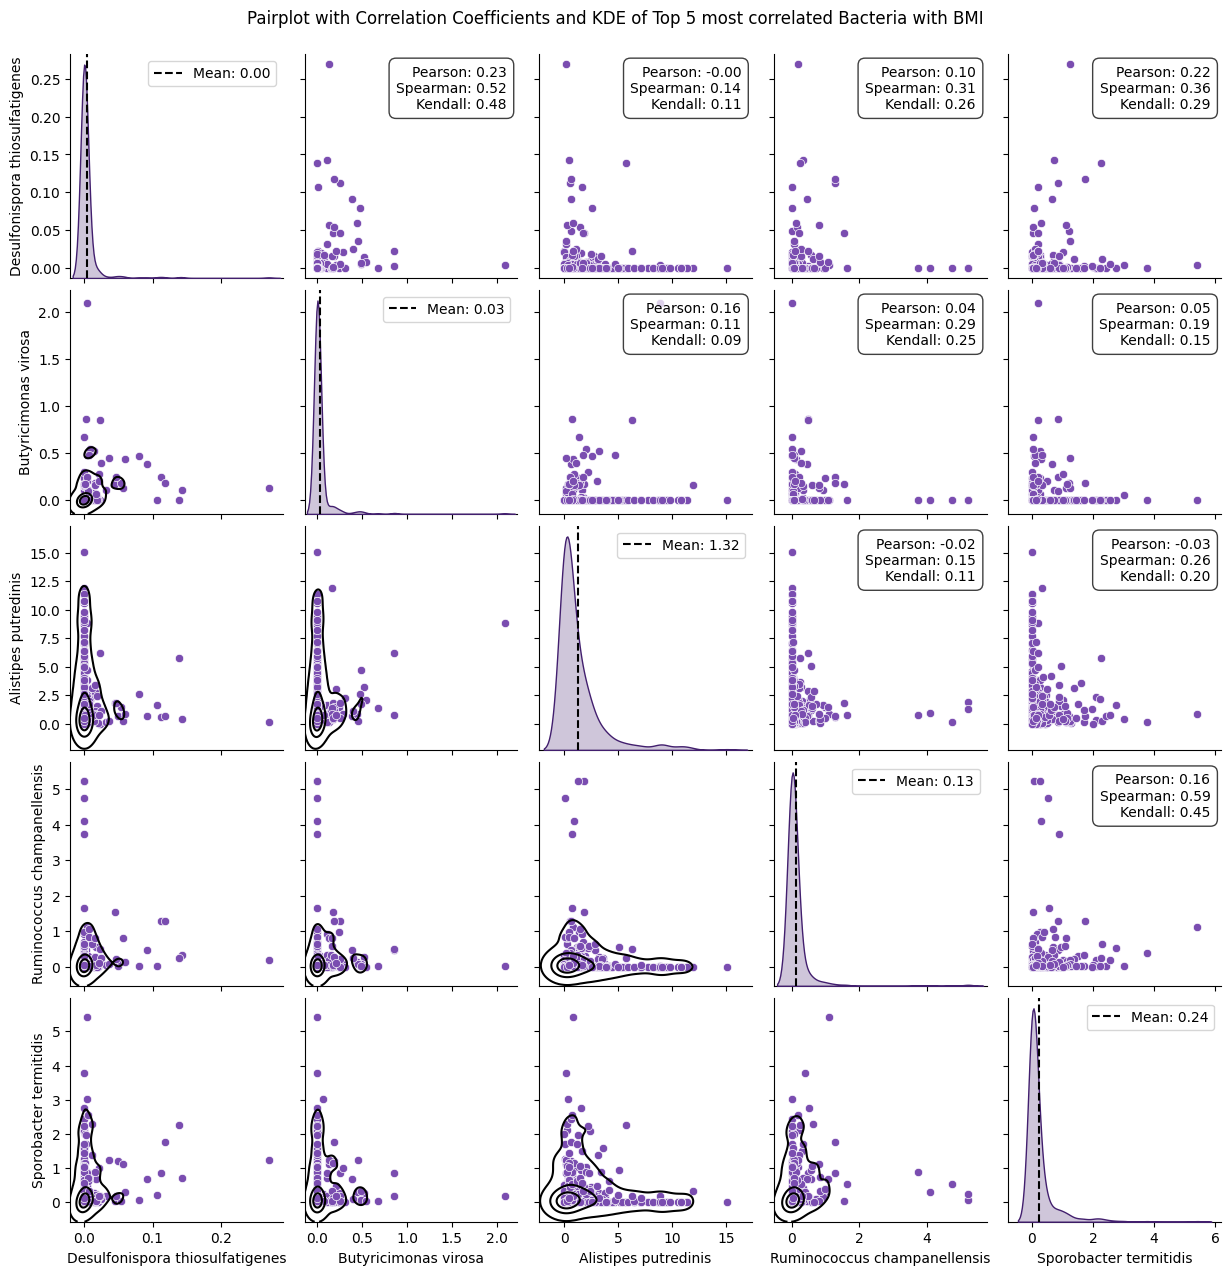
\includegraphics[width=\textwidth]{ims/corr_coeffs_top_5.png}
    \caption{Pairplot of the top $5$ bacteria based on correlation with BMI, plotted
    against each other.}
    \label{fig:corrs_top_5}
\end{figure}

One final attempt to capture the inner structure of our features is to use
dimensionality reduction techniques to try and project the data in a way that
would be beneficial to us. For example, using PCA, one can find the orthogonal
axes that span the directions of maximum variance in the data, allowing us to
reduce redundancy and potentially visualize high-dimensional patterns in a
lower-dimensional space. After performing PCA, I retained the first $5$ principal
components and plotted them in pairs, Figure~\ref{fig:PCA}. The same process
was followed with t-SNE and UMAP (\textit{the results can be seen in the notebook}
\texttt{data\_exploration.ipynb}\textit{, they will not be included here as their
results are similar to the ones already presented}). No matter the technique used,
no discernible structure can be observed.

\begin{figure}[H]
    \centering
    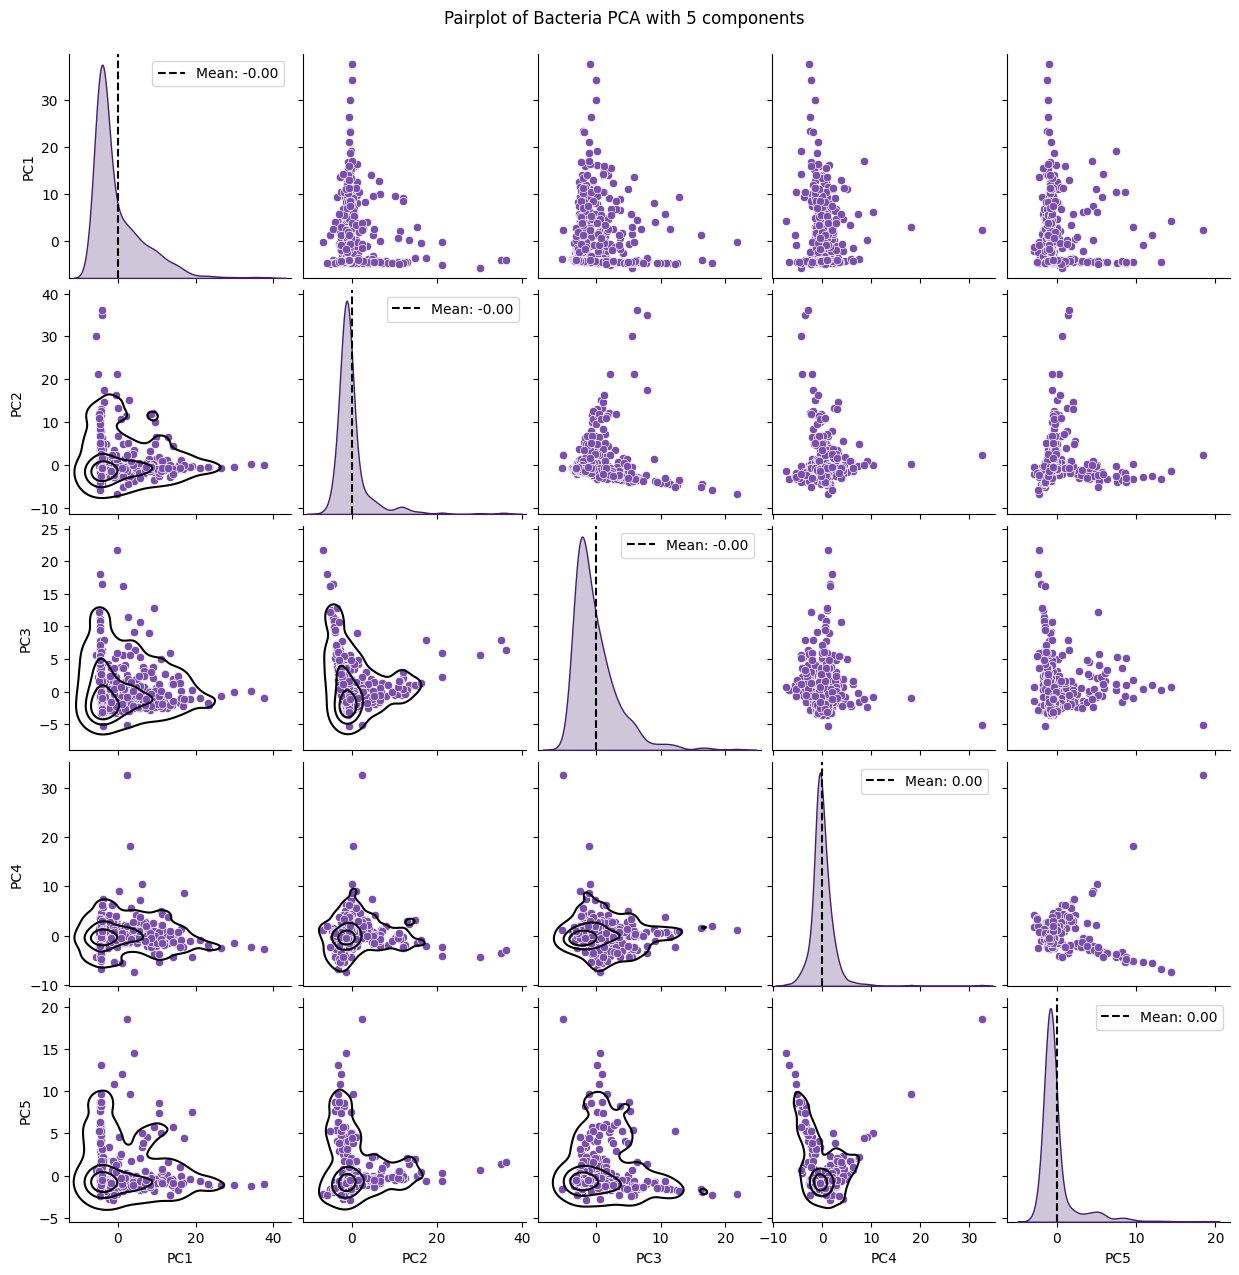
\includegraphics[width=\textwidth]{ims/PCA.png}
    \caption{PCA: Pairplot of the first 5 principal components.}
    \label{fig:PCA}
\end{figure}


\subsection{Conclusion}
\begin{enumerate}
    \item First we can observe that BMI (dependent variable) does not follow the
    normal distribution, so a simple linear regression model like the least squares
    will likely not work. One interesting thing to notice is that the male
    participants have a higher BMI than the female participants, which will likely
    play a role in the final model.
    \item When plotting the number of bacteria with zero values and the mean BMI
    when the bacteria are not zero we get something interesting. The bacteria with
    many zero values, show a different BMI compared to the rest.
    \item The bacteria lie close to $0$ with only a few outliers as seen by their
    means and Inter Quantile Ranges (IQR). A MinMax normalization would make the
    features very sparce in the range $[0, 1]$, so a Standardization seems like a
    better approach.
    \item Using Pearson's r, Spearman's $\rho$, and Kendall's $\tau$ correlation
    coefficients we see that there is not a single bacterial species that is highly
    correlated (either positively or negatively) with BMI. Plotting a pairplot of
    the $5$ most correlated features with BMI we can see that those features are
    not highly correlated between themselves so at least they --in theory-- carry
    different information and using them would be helpful.
    \item When using either of the three dimensionality reduction methods (PCA,
    t-SNE, UMAP) no visible clusters form.
\end{enumerate}


%%%%%%%%%%%%%%%%%%%%%%%%%%%%%%%%%%%%%%%%%%%%%%%%%%%%%%%%%%%%%%%%%%%%%%%%%%%%%%%%%%%%
\section{Regression}
\subsection{Baseline models}

The first step in the regression task is to create a baseline model. I created three
baseline models, one for each type of regressor: Elastic Net, SVR, and Bayesian
Ridge. The model training was performed by first fitting a standardizer to the 
training set (after splitting the data into training and testing sets) and then
transforming the training and testing sets. The models were trained using the
training set with no cross-validation, and the results were evaluated using the
testing set.


\subsection{Feature selection}
The next step was to perform feature selection and train the models again, using the
selected features. I decided to use a method that is model-dependent, so for each
of the three model types, I performed feature selection using different methods, then
I calculated the scores of the models using the selected features and I chose the
best performing feature selection method for each model.

The feature selection methods I used are:
\begin{itemize}
    \item \textbf{SelectKBest}: I used the \texttt{SelectKBest} method to select the
    top $k$ features based on two different metrics:
    \begin{itemize}
        \item \texttt{f\_regression}: This method uses the F-statistic to select
        the features.
        \item \texttt{r\_regression}: This method uses the Pearson's r
        correlation coefficient to select the features.
    \end{itemize}
    \item \textbf{VarianceThreshold}: I used the \texttt{VarianceThreshold} method
    to select the features with the highest variance.
\end{itemize}

All methods are implemented in the \texttt{sklearn} library. The first step of the
process is to perform feature selection using these methods and then train the
models using the selected features using a K Fold cross-validation with $5$ folds.
After that, I selected the method that yielded the best score for each model, based
on the following scoring function (Equation~\ref{eq:score}).
\begin{equation}    
\text{score} = \frac{
    \text{mean}(R^2)
    }{
    (\text{mean}(RMSE) + \text{mean}(MAE)) / 2
    }
    \label{eq:score}
\end{equation}

I used this scoring function to try and balance the maximization of the $r^2$ score
with the minimization of RMSE and MAE. The selected feature selection methods for
each model are:
\begin{itemize}
    \item \textbf{Elastic Net}: \texttt{SelectKBest} with the \texttt{f\_regression}
    metric and $k=20$, yielding $20$ features.
    \item \textbf{SVR}: \texttt{SelectKBest} with the \texttt{r\_regression} metric
    and $k=20$, yielding $20$ features.
    \item \textbf{Bayesian Ridge}: \texttt{VarianceThreshold} with a threshold of
    $0.5$, yielding $26$ features.
\end{itemize}

The selected features for each model are shown in Figure~\ref{fig:selected_features}.
The features are sorted by the times they were selected by for each model type. As
was expected, \textit{Host age} was selected for all models, but \textit{Sex} was
not selected by \texttt{SVR} which used the \texttt{r\_regression} metric.

\begin{figure}[H]
    \centering
    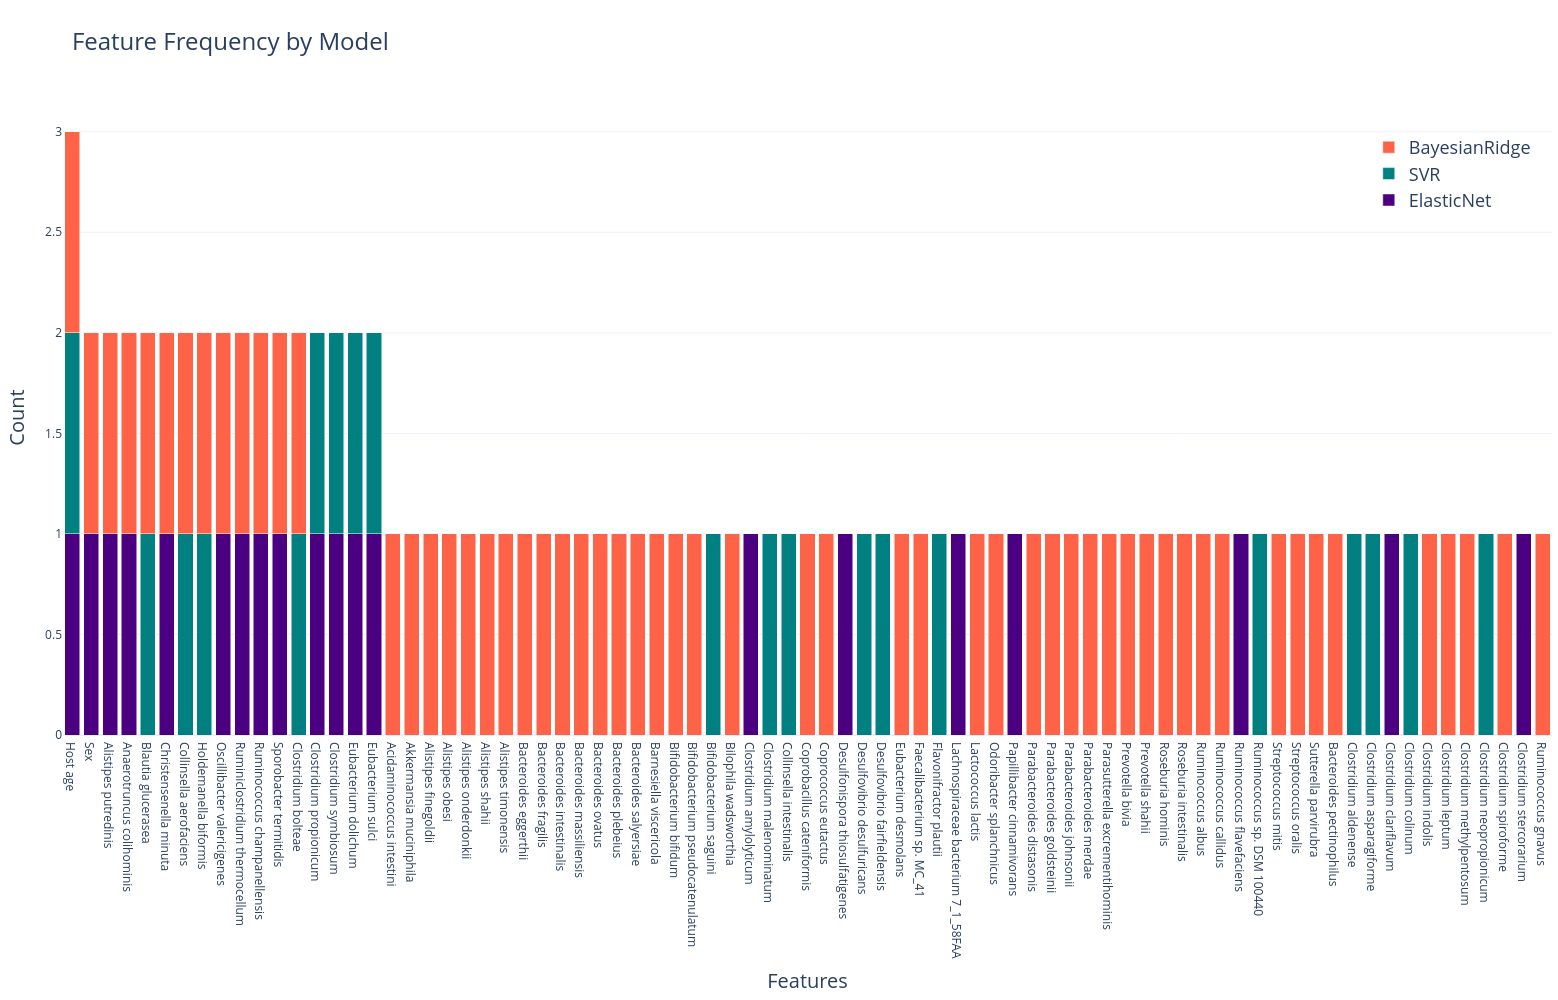
\includegraphics[width=\textwidth]{ims/selected_features.png}
    \caption{Selected features for each model. }
    \label{fig:selected_features}
\end{figure}


\subsection{Tuning}
The final step was to tune the models using the selected features. I used a
\texttt{GridSearchCV} with $5$ folds with negative mean squared error, negative
mean absolute error, and $R^2$ as scoring metrics.

The hyperparameter spaces for each model are summarized in the following table (%
Table~\ref{tab:hyperparams}).
    
\begin{table}[H]
    \centering
    \begin{tabular}{|c|c|c|c|}
        \hline
        \textbf{Model} & \textbf{Parameter} & \textbf{Values} & \textbf{Picked value} \\
        \hline
        \multirow{3}{*}{ElasticNet} 
            & \texttt{$\alpha$} & \texttt{linspace}(0.1, 1.0, \texttt{grid\_size}) & 0.98 \\
            & \texttt{l1 ratio} & \texttt{linspace}(0.1, 1.0, \texttt{grid\_size}) & 0.1 \\
            & \texttt{tolerance} & [1e-3, 1e-4, 1e-5, 1e-6, 1e-7] & 0.001 \\
        \hline
        \multirow{7}{*}{SVR} 
            & \texttt{kernel} & [`rbf', `linear', `poly', `sigmoid'] & `rbf' \\
            & \texttt{degree} & [2, 3, 4] & 2 \\
            & \texttt{$\gamma$} & [`scale', `auto'] & `auto' \\
            & \texttt{coef\_0} & \texttt{linspace}(0.0, 1, \texttt{grid\_size}) & 0.0 \\
            & \texttt{tolerance} & [1e-3, 1e-4, 1e-5, 1e-6, 1e-7] & 1e-7 \\
            & \texttt{C} & \texttt{linspace}(0.1, 1.0, \texttt{grid\_size}) & 1 \\
            & \texttt{$\epsilon$} & \texttt{linspace}(0.0, 1.0, \texttt{grid\_size}) & 0.222 \\
        \hline
        \multirow{6}{*}{BayesianRidge} 
            & \texttt{tolerance} & [1e-3, 1e-4, 1e-5, 1e-6, 1e-7] & 0.001 \\
            & \texttt{$\alpha_1$} & \texttt{linspace}(1e-3, 1e-9, \texttt{grid\_size}) & 0.001 \\
            & \texttt{$\alpha_2$} & \texttt{linspace}(1e-3, 1e-9, \texttt{grid\_size}) & 1e-9 \\
            & \texttt{$\lambda_1$} & \texttt{linspace}(1e-3, 1e-9, \texttt{grid\_size}) & 1e-9 \\
            & \texttt{$\lambda_2$} & \texttt{linspace}(1e-3, 1e-9, \texttt{grid\_size}) & 0.001 \\
            & \texttt{compute\_score} & [True, False] & True \\
        \hline
    \end{tabular}
    \caption{Hyperparameter spaces for each model. The \texttt{grid\_size} is the
    number of points in the grid for each hyperparameter, set to $50$ by default.
    The \texttt{linspace} function used provided by \texttt{numpy} is returning
    evenly spaced numbers over a specified interval. The values are presented exactly
    as they were passed in the \texttt{Python} functions for easier comparison
    with the code base.}
    \label{tab:hyperparams}
\end{table}


\subsection{Results}

The results of the whole process can be seen in the boxplots below (Figure~\ref{%
fig:elasticnet_results}, Figure~\ref{fig:svr_results}, and Figure~\ref{%
fig:bayesianridge_results}). The models, after being trained with the development
set, were tested on teh validation set. For a better calculation of metrics, I opted
to using bootstrapping/resampling. Resampling, as the name implies, resamples
(randomly) values from the data set in each different loop, leading to different
combinations of the data set; I used $1000$ loops, so the below boxplots show the
metrics calculated $1000$ times with resampling.

\begin{figure}[H]
    \centering
    \begin{subfigure}{0.3\textwidth}
        \centering
        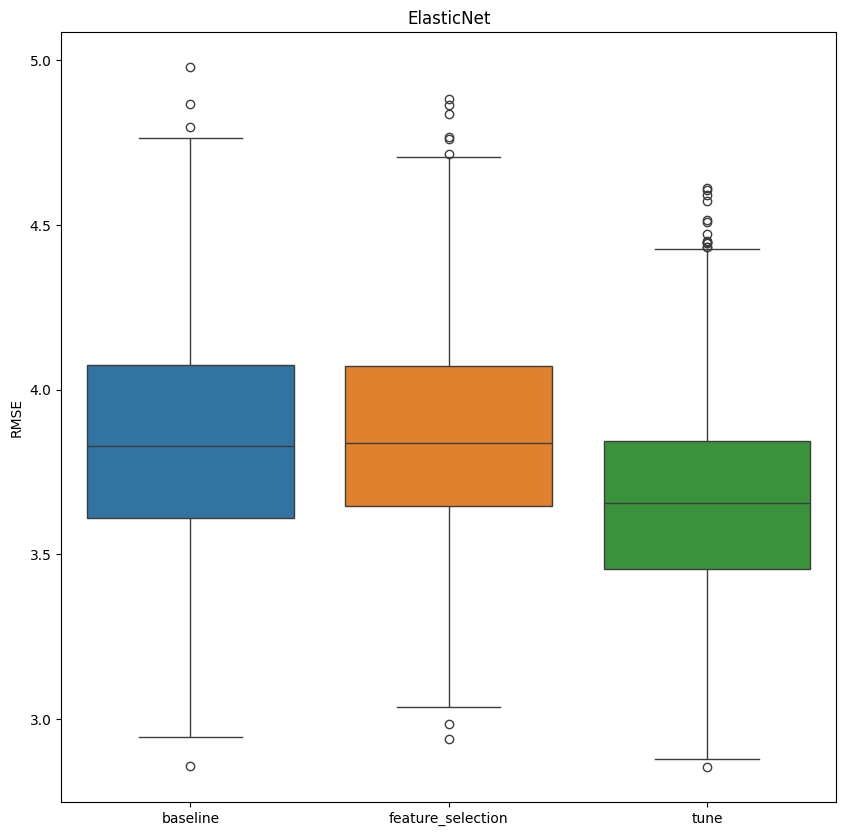
\includegraphics[width=\linewidth]{ims/elasticnet_rmse.png}
        \caption{RMSE}
        \label{fig:elasticnet_rmse}
    \end{subfigure}
    \begin{subfigure}{0.3\textwidth}
        \centering
        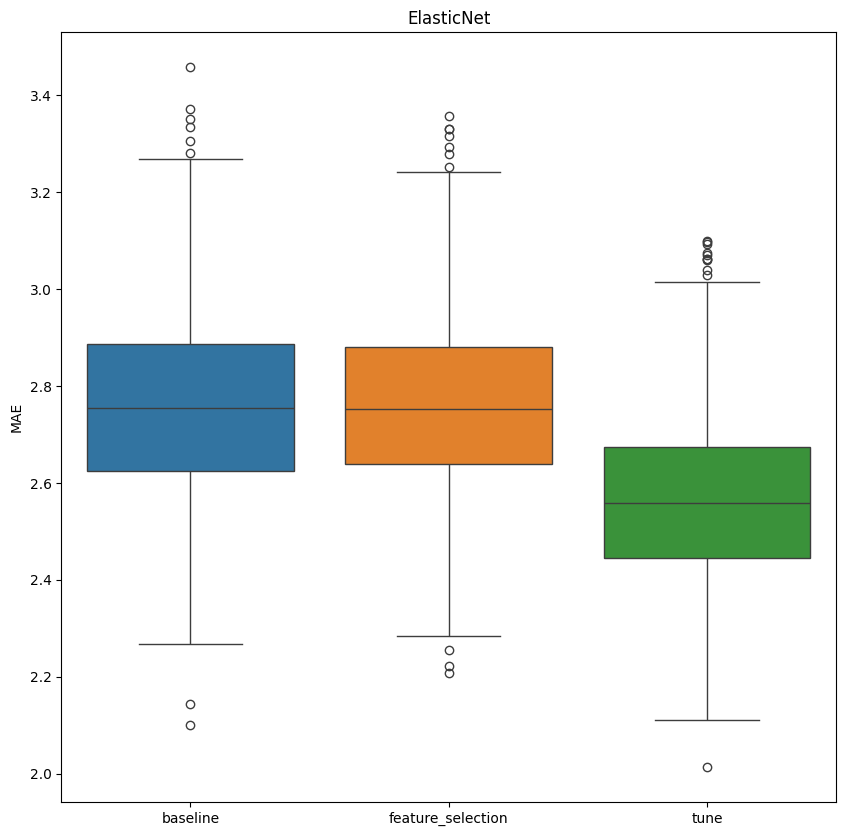
\includegraphics[width=\linewidth]{ims/elasticnet_mae.png}
        \caption{MAE}
        \label{fig:elasticnet_mae}
    \end{subfigure}
    \begin{subfigure}{0.3\textwidth}
        \centering
        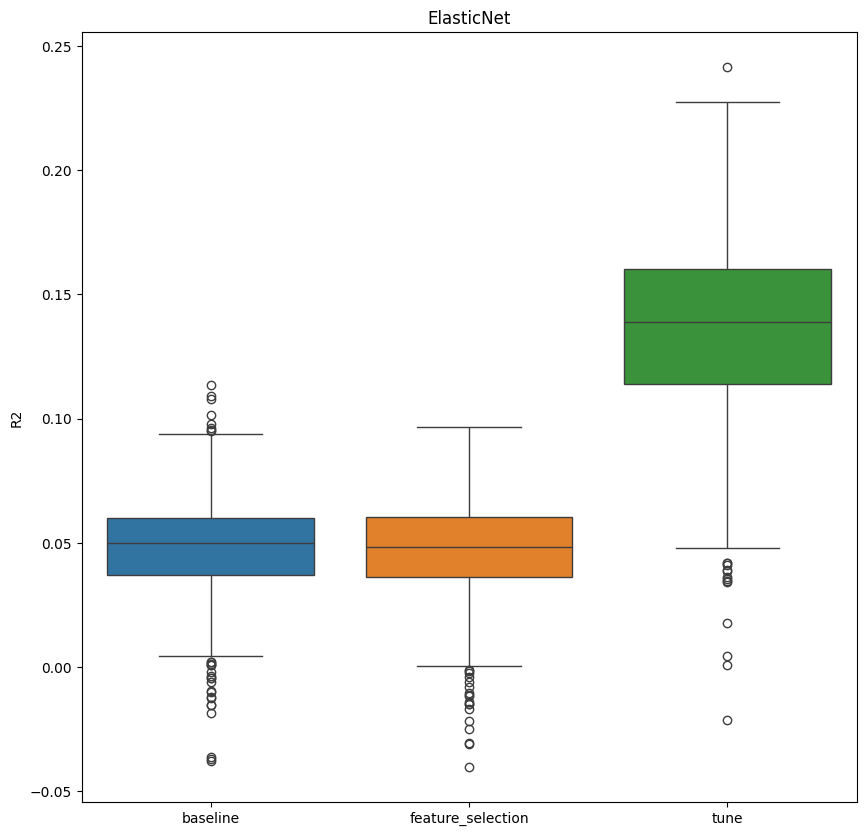
\includegraphics[width=\linewidth]{ims/elasticnet_r2.png}
        \caption{$R^2$}
        \label{fig:elasticnet_r2}
    \end{subfigure}
    \caption{Elastic Net: Results based on the validation set, RMSE, MAE, and $R^2$.
    Blue box for the baseline model, orange box for the feature selection model, and
    green box for the tuned model.}
    \label{fig:elasticnet_results}
\end{figure}

\begin{figure}[H]
    \centering
    \begin{subfigure}{0.3\textwidth}
        \centering
        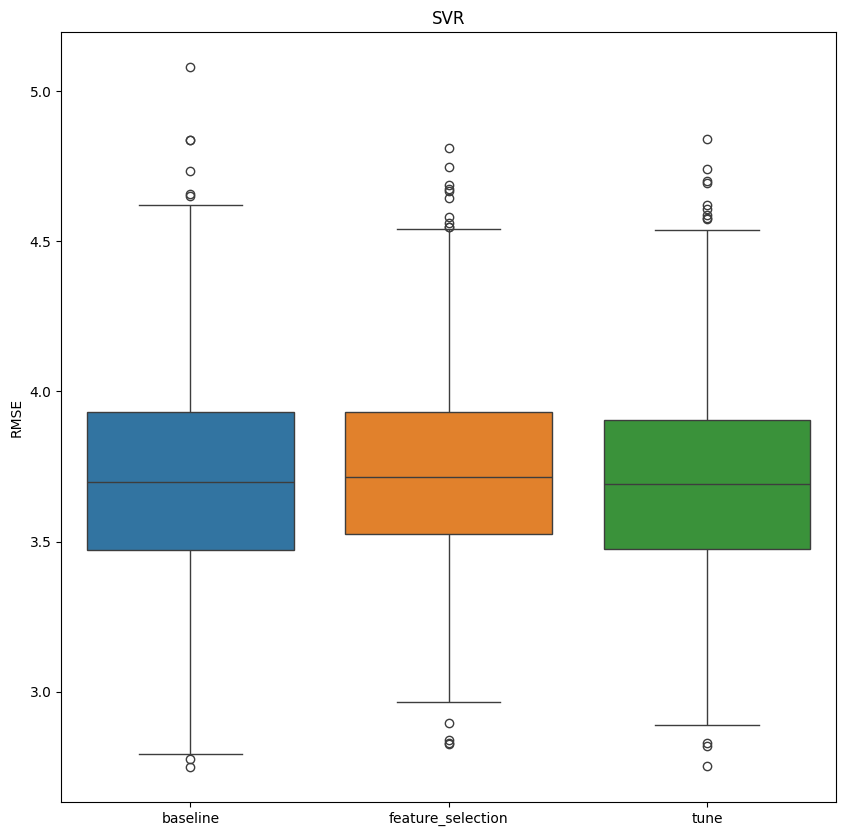
\includegraphics[width=\linewidth]{ims/svr_rmse.png}
        \caption{RMSE}
        \label{fig:svr_rmse}
    \end{subfigure}
    \begin{subfigure}{0.3\textwidth}
        \centering
        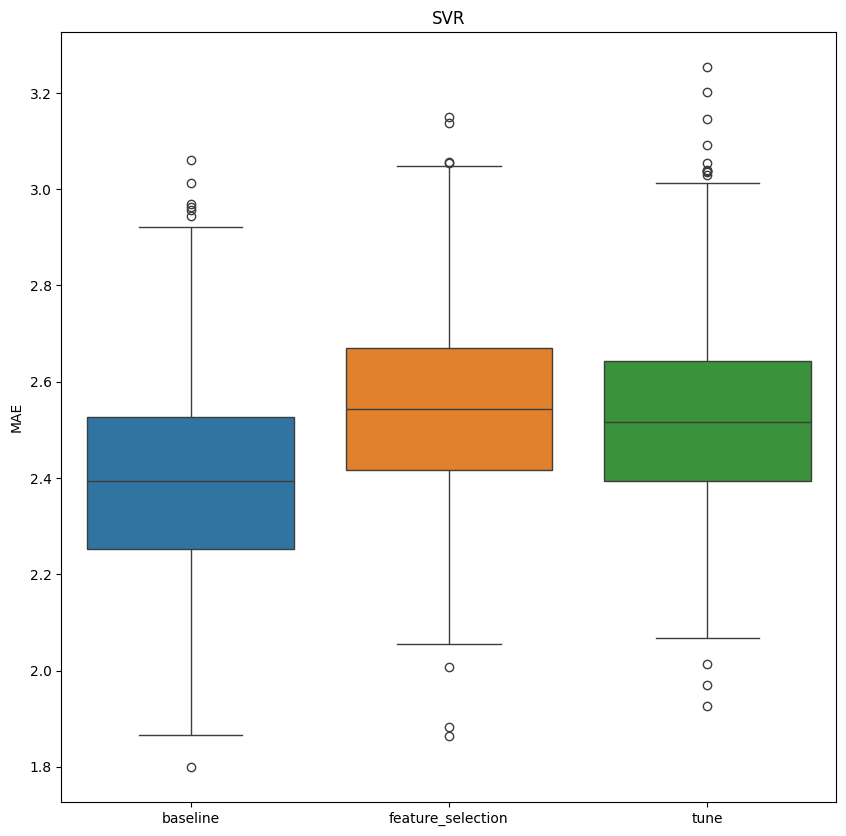
\includegraphics[width=\linewidth]{ims/svr_mae.png}
        \caption{MAE}
        \label{fig:svr_mae}
    \end{subfigure}
    \begin{subfigure}{0.3\textwidth}
        \centering
        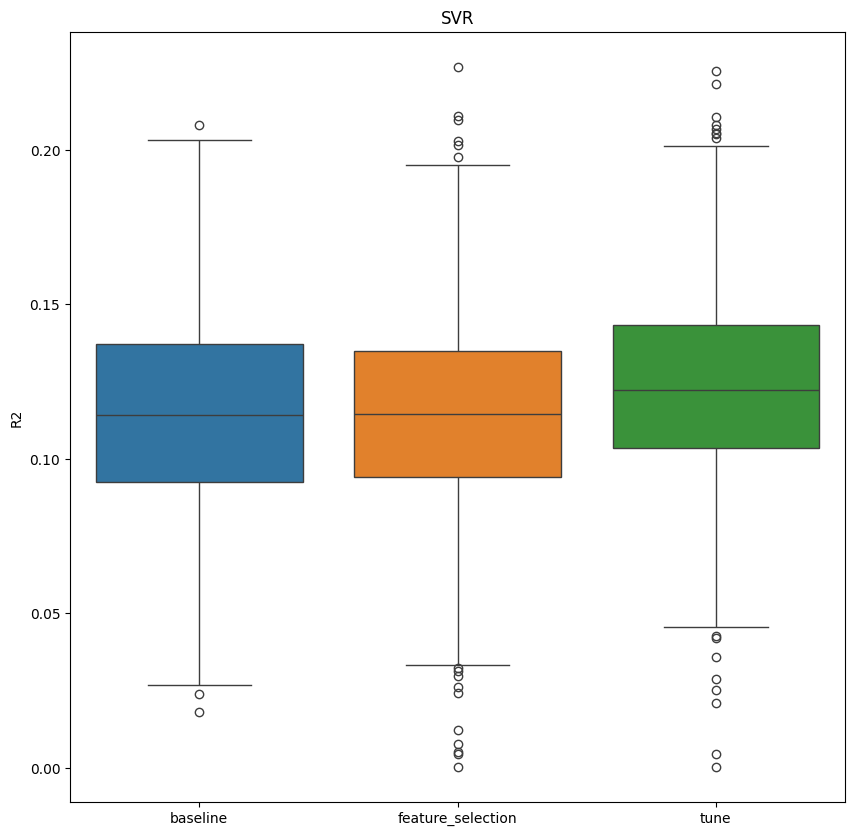
\includegraphics[width=\linewidth]{ims/svr_r2.png}
        \caption{$R^2$}
        \label{fig:svr_r2}
    \end{subfigure}
    \caption{SVR: Results based on the validation set, RMSE, MAE, and $R^2$. Blue
    box for the baseline model, orange box for the feature selection model, and green
    box for the tuned model.}
    \label{fig:svr_results}
\end{figure}

\begin{figure}[H]
    \centering
    \begin{subfigure}{0.3\textwidth}
        \centering
        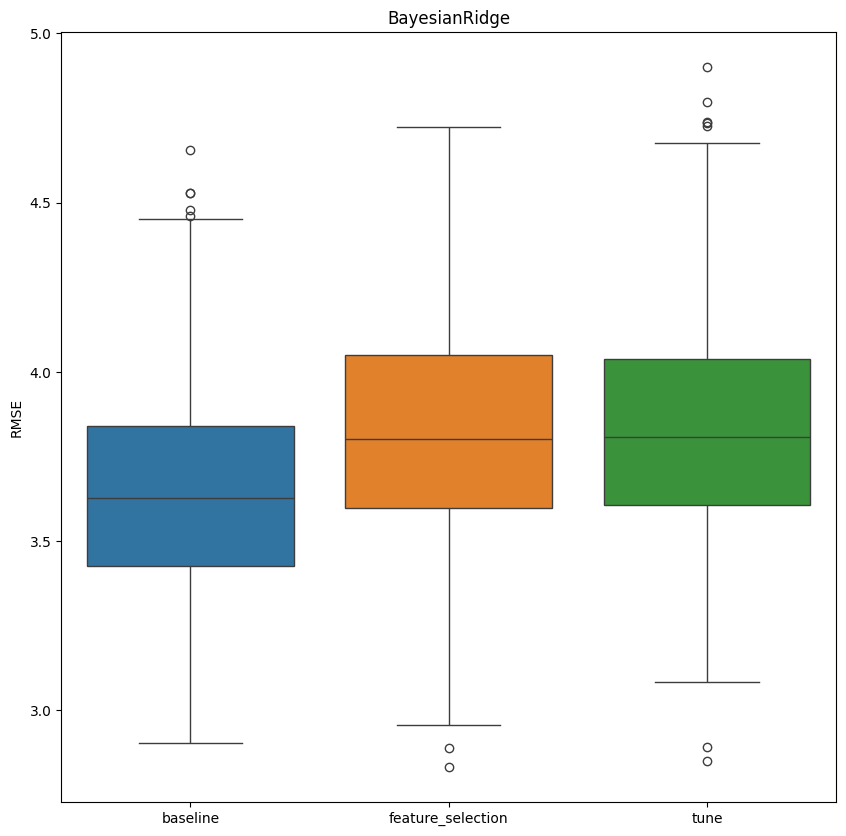
\includegraphics[width=\linewidth]{ims/bayesianridge_rmse.png}
        \caption{RMSE}
        \label{fig:bayesianridge_rmse}
    \end{subfigure}
    \begin{subfigure}{0.3\textwidth}
        \centering
        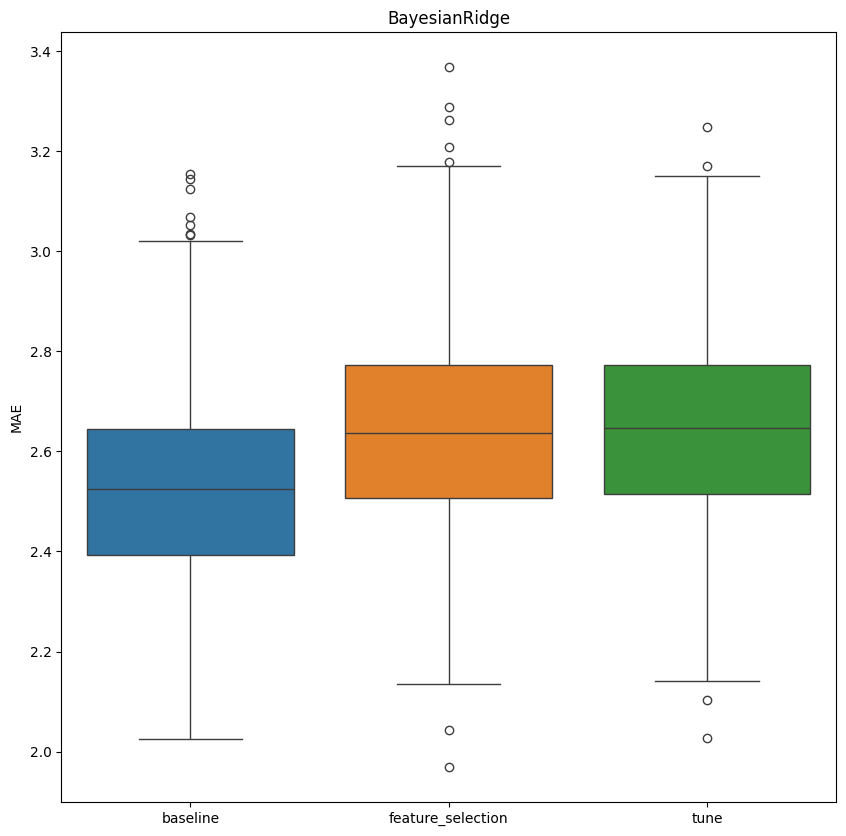
\includegraphics[width=\linewidth]{ims/bayesianridge_mae.png}
        \caption{MAE}
        \label{fig:bayesianridge_mae}
    \end{subfigure}
    \begin{subfigure}{0.3\textwidth}
        \centering
        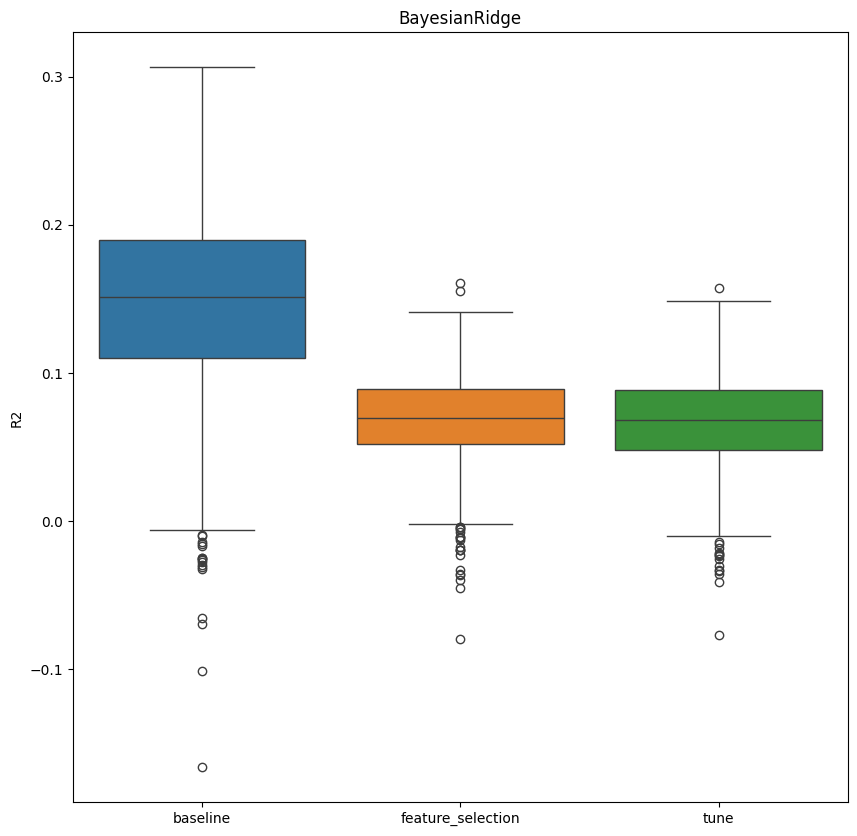
\includegraphics[width=\linewidth]{ims/bayesianridge_r2.png}
        \caption{$R^2$}
        \label{fig:bayesianridge_r2}
    \end{subfigure}
    \caption{Bayesian Ridge: Results based on the validation set, RMSE, MAE, and
    $R^2$. Blue box for the baseline model, orange box for the feature selection
    model, and green box for the tuned model.}
    \label{fig:bayesianridge_results}
\end{figure}

The first thing we notice, is that for all cases, either feature selection, or
tuning, leads to similar results as the baseline model. For some cases even, the
models seem to perform worse after tuning or feature selection (for example SVR has
higher MAE, Figure~\ref{fig:svr_mae}; Bayesian Ridge has smaller $R^2$, Figure~\ref{%
fig:bayesianridge_r2}).

The scores for all models are very similar, with RMSEs between $3.5$ and $4$, MAEs
around $2.6$, and $R^2$ scores between $0$ and $0.2$. Elastic Net seems to be the
only model that displays any improvement after tuning. SVR shows similar scores,
while Bayesian Ridge shows worse scores after tuning.

The model I select as the \textbf{best}, considering it's speed, predictive ability
and simplicity is \textbf{Elastic Net} with feature selection and tuning.

\end{document}